% generated by scripts/pkl_to_latex.py
% source PKL : vscan_v1_L8_Ne8_U10_t1_mode-uniform_nmin2_solver-gcg_full_restarts10_iter300_kmax5_tol1em09_V0to12_N25-ebabade1a2a1.pkl
% scan type  : vscan
% state      : gs
% quantity   : cgme
% requires   : \usepackage{pgfplots} \pgfplotsset{compat=1.18}
% colours match the matplotlib PDF (tab10 cycle)
\definecolor{gmeC0}{HTML}{1F77B4}
\definecolor{gmeC1}{HTML}{FF7F0E}
\definecolor{gmeC2}{HTML}{2CA02C}
\definecolor{gmeC3}{HTML}{D62728}
\definecolor{gmeC4}{HTML}{9467BD}
\definecolor{gmeC5}{HTML}{8C564B}
\definecolor{gmeC6}{HTML}{E377C2}
\definecolor{gmeC7}{HTML}{17BECF}

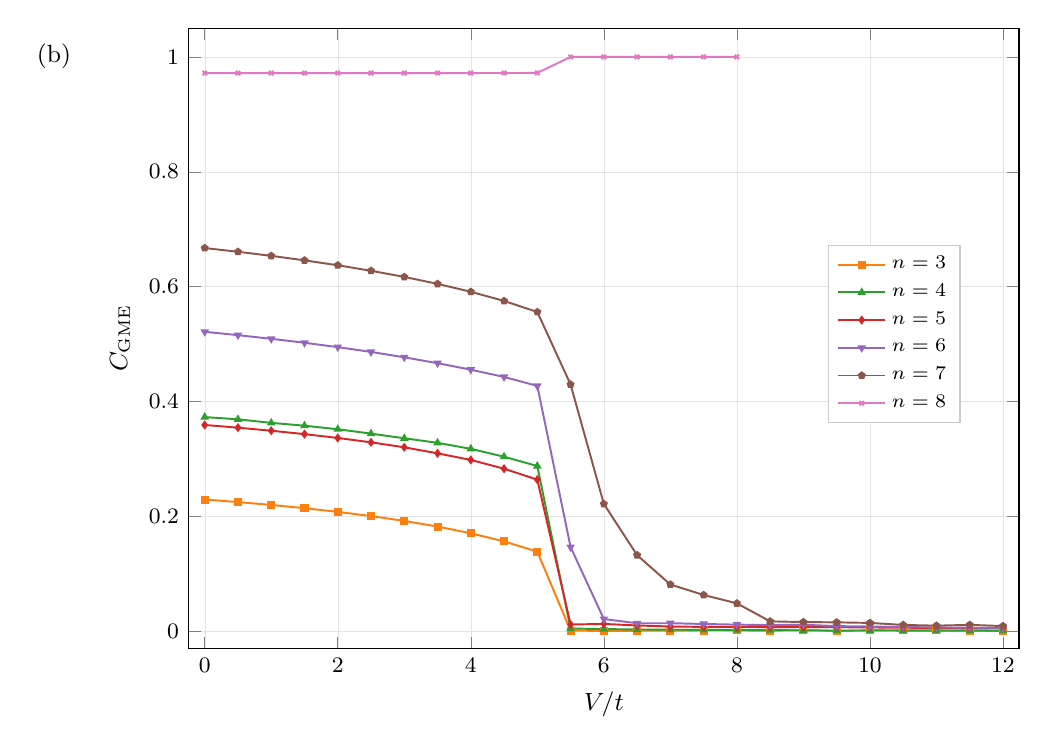
\begin{tikzpicture}
  \begin{axis}[
    width=\columnwidth,
    height=0.78\columnwidth,
    xlabel={$V/t$},
    ylabel={$C_{\mathrm{GME}}$},
    grid=both,
    grid style={line width=.1pt, draw=gray!20},
    tick label style={font=\footnotesize\rmfamily, /pgf/number format/fixed},
    label style={font=\small\rmfamily},
    scaled ticks=false,
    legend style={font=\scriptsize\rmfamily, draw=gray!40, at={(0.5,1.03)}, anchor=south, /tikz/every even column/.append style={column sep=6pt}},
    legend cell align={left},
    legend columns=1,
    ymin=-0.03,
    ymax=1.05,
    xmin=-0.24,
    xmax=12.24,
    legend style={at={(0.850,0.507)}, anchor=center, fill=white},
    after end axis/.append code={\node[anchor=east, font=\small\rmfamily] at (axis description cs:-0.13,0.954) {(b)};},
  ]
    \addplot[color=gmeC1, mark=square*, mark size=1.1pt, line width=0.7pt] coordinates {
        (0,0.229253) (0.5,0.22481) (1,0.219812) (1.5,0.214166)
        (2,0.207754) (2.5,0.200426) (3,0.191984) (3.5,0.182148)
        (4,0.170501) (4.5,0.156349) (5,0.138365) (5.5,0.001076)
        (6,0.00029) (6.5,0.000674) (7,0.00092) (7.5,0.001157)
        (8,0.00126) (8.5,0.000822) (9,0.00161) (9.5,0.00051)
        (10,0.001233) (10.5,0.001245) (11,0.00132) (11.5,0.000794)
        (12,0.000563)
    };
    \addlegendentry{$n=3$}
    \addplot[color=gmeC2, mark=triangle*, mark size=1.1pt, line width=0.7pt] coordinates {
        (0,0.372851) (0.5,0.368943) (1,0.362756) (1.5,0.357806)
        (2,0.351628) (2.5,0.344042) (3,0.335913) (3.5,0.328038)
        (4,0.317531) (4.5,0.303778) (5,0.287593) (5.5,0.004616)
        (6,0.00364) (6.5,0.003021) (7,0.002497) (7.5,0.002354)
        (8,0.001778) (8.5,0.001779) (9,0.001561) (9.5,0.000885)
        (10,0.001352) (10.5,0.00105) (11,0.00111) (11.5,0.000812)
        (12,0.000835)
    };
    \addlegendentry{$n=4$}
    \addplot[color=gmeC3, mark=diamond*, mark size=1.1pt, line width=0.7pt] coordinates {
        (0,0.359106) (0.5,0.354363) (1,0.34908) (1.5,0.343148)
        (2,0.336484) (2.5,0.328864) (3,0.320202) (3.5,0.309682)
        (4,0.298189) (4.5,0.282888) (5,0.26385) (5.5,0.011578)
        (6,0.012632) (6.5,0.009905) (7,0.00815) (7.5,0.007386)
        (8,0.007498) (8.5,0.007042) (9,0.007262) (9.5,0.006937)
        (10,0.006455) (10.5,0.006026) (11,0.005462) (11.5,0.004886)
        (12,0.005155)
    };
    \addlegendentry{$n=5$}
    \addplot[color=gmeC4, mark=triangle*, mark size=1.1pt, mark options={rotate=180}, line width=0.7pt] coordinates {
        (0,0.52136) (0.5,0.515491) (1,0.509151) (1.5,0.502245)
        (2,0.494636) (2.5,0.486321) (3,0.476906) (3.5,0.466689)
        (4,0.455367) (4.5,0.442726) (5,0.427122) (5.5,0.146421)
        (6,0.02113) (6.5,0.013795) (7,0.013858) (7.5,0.012549)
        (8,0.011392) (8.5,0.010596) (9,0.011181) (9.5,0.00882)
        (10,0.008103) (10.5,0.007148) (11,0.006601) (11.5,0.006095)
        (12,0.005237)
    };
    \addlegendentry{$n=6$}
    \addplot[color=gmeC5, mark=pentagon*, mark size=1.1pt, line width=0.7pt] coordinates {
        (0,0.66716) (0.5,0.660692) (1,0.653599) (1.5,0.645799)
        (2,0.63718) (2.5,0.627606) (3,0.616899) (3.5,0.604826)
        (4,0.591051) (4.5,0.575043) (5,0.555831) (5.5,0.429598)
        (6,0.221592) (6.5,0.132399) (7,0.081252) (7.5,0.063025)
        (8,0.048431) (8.5,0.017078) (9,0.015891) (9.5,0.015352)
        (10,0.014364) (10.5,0.010851) (11,0.00962) (11.5,0.010999)
        (12,0.008853)
    };
    \addlegendentry{$n=7$}
    \addplot[color=gmeC6, mark=x, mark size=1.1pt, line width=0.7pt] coordinates {
        (0,0.97189) (0.5,0.971891) (1,0.971892) (1.5,0.971895)
        (2,0.971898) (2.5,0.971903) (3,0.971911) (3.5,0.971925)
        (4,0.97195) (4.5,0.972001) (5,0.972117) (5.5,1)
        (6,1) (6.5,1) (7,1) (7.5,1)
        (8,1)
    };
    \addlegendentry{$n=8$}
  \end{axis}
\end{tikzpicture}
